\section{Backbone \texttt{model.save(\{\}, options)} failure}
A summary of the Stack Overflow question\cite{so_model_save} that Sarah posted is given below.
When trying to save a model and making use of \verb!success! and \verb!error! callbacks the documentation states that you can save a model with a call structure \verb!model.save([attributes], [options])!. 
It is not made clear in the documentation how to save the entire model (rather than listing the individual fields that have changed). We needed this in order to be able to save new models, for example in the student sign up, rather than listing every single individual field we wanted to save them all.
Another Stack Overflow question\cite{so_save_all_fields} was found that told us in order to do this we could call \verb!model.save({}, [options])!.

However when saving the model we noticed that the error callback was always being called rather than the success, even though the server was returning OK.

With some logging in the console we realised that the model was indeed infact valid before and after the call to save, but the error response message was that all of the fields were required (which on logging the model we could see they were there).

This was very puzzling and so we had to investigate via the backbone code documentation\cite{backbone_code} and the changelog of the latest version release\cite{backbone_change_log} to find out that they had updated what happens if you pass \verb!wait: true! into the save options.

The documentation details `Pass \verb!{wait: true}! if you'd like to wait for the server before setting the new attributes on the model', which to us seemed like exactly what we wanted. 
However on inspecting the documented code , what actually happens is the attributes will be reset to the server values via a call to clear the model, and then a call to set the options.
It is on this \verb!clear! call that our error callback was being called, since we have validation in all of our models
to document which fields are required. By clearing a field it will not pass validation and so this is where the mysterious message that the attribtues must be set was coming from.

\begin{figure}[H]\centering
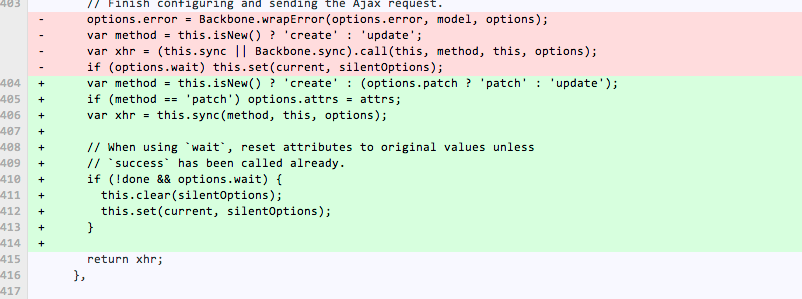
\includegraphics[scale=0.5]{images/appendix/backbone_changelog}
\caption{Changelog for save method. Clearly shows clear has been added.}
\end{figure}

In order to fix this issue we decided to set \verb!forceUpdate: true! as an option, instead of removing \verb!wait: true!, since we'd prefer to use server values if indeed they haven't changed. We decided forcing our Backbone model to update despite validation is alright in this situation because we know that the server has a higher level of validation and so our model will always infact be valid.

